\documentclass[a4paper,12pt]{article}
\usepackage[hidelinks]{hyperref}
\usepackage{float}
\usepackage{graphicx}
\usepackage{listings}
\usepackage[utf8]{inputenc}
\usepackage{etoolbox}
\usepackage{fullpage}
\renewcommand*\contentsname{Indice}
\renewcommand*\figurename{Fig.}
\usepackage{setspace}
\usepackage{parskip}
\usepackage{subfigure}
\usepackage{amsmath}


\makeatletter
\patchcmd\l@section{%
  \nobreak\hfil\nobreak
}{%
  \nobreak
  \leaders\hbox{%
    $\m@th \mkern \@dotsep mu\hbox{.}\mkern \@dotsep mu$%
  }%
  \hfill
  \nobreak
}{}{\errmessage{\noexpand\l@section could not be patched}}
\makeatother

\setcounter{secnumdepth}{0}

% un po' di estetica...
\usepackage{fancyhdr}
\pagestyle{fancy}
\setlength{\headsep}{0.35in}
\let\MakeUppercase\relax

% blocchi di codice
\usepackage{listings}
\lstset{
	breaklines=true, 
	frame=single, 
	numbers=left,
	tabsize=2,
	basicstyle=\scriptsize,
	showstringspaces=false
}

\setlength{\parindent}{2em}
\setlength{\parskip}{0.5em}
\renewcommand{\baselinestretch}{1.5}

\fancyhf{} % clear all fields
\fancyfoot[C]{\thepage}

\frenchspacing

\begin{document}

\begin{titlepage}
\noindent
    \vspace*{5mm}
	\begin{minipage}[t]{0.15\textwidth}
	    \vspace*{5mm}
		\vspace{-3.5mm}{
\includegraphics[scale=1.8]{img/logo_bicocca.png}}
	\end{minipage}
	\hspace{1cm}
	\begin{minipage}[t]{0.9\textwidth}
	      \vspace*{5mm}
		{
			\setstretch{1.42}
			{\textsc{Università degli Studi di Milano - Bicocca} } \\
			\textbf{Scuola di Scienze} \\
			\textbf{Dipartimento di Informatica, Sistemistica e Comunicazione} \\
			\textbf{Corso di Laurea Magistrale in Informatica} \\
			\par
		}
	\end{minipage}
	
	\vspace{42mm}

\begin{center}
    {\LARGE{
	    	\setstretch{2}
            \textbf{
            	Data Analytics \\ 
            	Sentiment Analysis and Network Analysis on Amazon}
    }}        
\end{center}

\vspace{40mm}
	
	
	\begin{flushright}
		\setstretch{1.3}
		\large{Cocca Umberto - 807191} 
	\end{flushright}
	
	\vspace{15mm}
	\begin{center}
		{\large{\bf Anno Accademico 2019 - 2020}}
	\end{center}


\renewcommand{\baselinestretch}{1.5}

\end{titlepage}

\tableofcontents

\newpage

\section{Introduzione}
Negli ulitmi anni si è visto un numero crescente di ricerche che hanno ampliato la comprensione del sentiment delle risorse testuali determinando l’avvento di servizi online che hanno cambiato
il volto allo shopping. 

\noindent Applicazioni di commercio online come Amazon concepiscono
una quantità spropositata di dati per mezzo delle transizioni e degli utenti di
questo servizio, infatti una parte consistente è data dai contenuti generati dagli
utenti che valutano i prodotti acquistati e condividono la loro esperienza procedendo con valutazioni numeriche, seguite spesso da delle recensioni.

\noindent La Sentiment Analysis estrae dei dati strutturati da queste risorse testuali, permettendo un'analisi statistica sulle tendenze di comunità di acquirenti sotto diversi aspetti. Le aziende vogliono sempre trovare opinioni ed emozioni del pubblico o dei loro consumatori sui loro prodotti e servizi. Non solo, anche i potenziali clienti vogliono conoscere le opinioni e le emozioni degli utenti che hanno già usufruito di un certo servizio o acquistato un certo prodotto. Conoscere gli elementi più o meno apprezzati di un prodotto, secondo le diverse categorie di utenti, permette di condurre una migliore previsione del mercato e quindi attuare strategie aziendali favorevoli. 

\noindent Le recensioni vengono recepite come fonti affidabili, rappresentando quindi uno strumento molto potente.
\bigskip

\noindent È possibile trovare il listato dei codici alla seguente \href{https://github.com/okamiRvS/Sentiment-Analysis-for-Amazon-Reviews}{\textbf{repository}}.


\newpage

\subsection{Sentiment Analysis}
Il Sentiment Analysis serve per interpretare il linguaggio naturale e identificare informazioni soggettive che denotano opinioni, emozioni e sentimenti, determinndo la polarità corrispondente (positiva, negativa o neutra) e comprendere il soggetto / oggetto target. 

\noindent In questa fase, viene analizzata sistematicamente le parti testuali delle recensioni per estrarne un’opinione.
Una parte preliminare pre-processing servirà per preparare il dataset. Vengono scartate recensioni troppo lunghe o troppe corte.

\noindent Infine, viene utilizzato ASUM (Aspet Sentiment Unification Model) per poter estrarre quelle che sono un insieme di topic che sono riferiti ai sentiment positivi e negativi. Usando ASUM si assume che il documento sia composto da frasi.
\bigskip

\subsection{Dataset}
Il dataset utilizzato è estratto da Amazon, in formato JSON, in cui sono presenti le recensioni rilasciate dagli utenti sul sito. Dal dataset si è specializzato per la categoria videogiochi.

\section{Software utilizzati}
Il flusso di lavoro si compone di due aree, una fase di manipolazione dei dati attraverso Python e una fase di processione dei dati attraverso il modello ASUM per il sentiment analysis.

\subsection{Python}
Per eseguire il preprocessing si è lavorato con Python, scelta dovuta alla
grande quantità di strumenti e librerie open source disponibili per questo linguaggio. Le librerie utilizzate sono le seguenti:
\begin{itemize}
	\item \textit{Pandas}: per caricare e manipolare il dataset
	\item \textit{NLTK}: per separare ogni review in una lista di frasi
	\item \textit{re}: per eseguire una pulizia parziale sui dati, ad esempio eliminando quelle parole composte solo da numeri, o da caratteri inadeguati.  
\end{itemize}

\subsection{ASUM}
Per mezzo di Python si è costruito l'input ad hoc per la versione Java di ASUM creata da Yohan Jo and Alice Oh, consultabile al seguente \href{http://www.cs.cmu.edu/~yohanj/research/WSDM11/index.html}{\textbf{link}}.

\noindent L'input del programma è costituito da tre file, due obbligatori e uno opzionale:
\begin{itemize}
	\item \textit{BagOfSentences.txt} (obbligatorio)\\ 
	Questo file è una rappresentazione dell'elenco di parole dei documenti nel corpus.
	Per ogni documento, la prima riga è il numero di frasi. Dalla riga successiva viene visualizzato un elenco di indici che si riferiscono alla posizione relativa nel WordList;
	\item \textit{WordList.txt} (obbligatorio)\\
	Questo file mappa le parole con indici di parole. Ogni parola è scritta in una riga. Si presume che la prima parola nel file abbia l'indice 0, la seconda parola abbia indice 1 e così via...;
	\item \textit{SentiWords-0.txt, SentiWords-1.txt, … } (opzionale)\\
	Questi file sono parole chiamati "semi sentimentali". Il numero del file dovrebbe iniziare da 0 e aumentare gradualmente. Nel modello ASUM è possibile aiutare il processo di campionamento facendo uso di queste informazioni a priori. Se sappiamo che una determinata parola è positiva perché appartiene al lessico dei positivi allora la sua probabilità di essere positiva la si conosce. 
	
	Nello specifico per il progetto si sono usati due sentiment, uno positivo e uno negativo sfruttando due liste di parole italiane recuperate dal seguente \href{https://github.com/gragusa/sentiment-lang-italian}{\textbf{link}} e manipolato leggermente aggiungendo alcune emoticon testuali.
\end{itemize}

\newpage

\subsection{Specializzazione del dataset}
Vista la quantità considerabile dei dati per via del numero di utenti e del numero di prodotti (nell’ordine del milione) è complicato fare analisi esplorative approfondite su ogni singolo utente e su ogni singolo prodotto. 
Visto l'enorme quantità di dati si è selezionata una categoria ben specifica per il processamento dei dati: videogiochi.
\bigskip

\subsection{Descrizione dataset}
Il dataset è in formato JSON e viene caricato in memoria in formato DataFrame, con la libreria Pandas, in modo molto efficiente nonostante il dataset sia composto da circa due milioni di recensioni. 

\noindent Infatti, il caricamento e il pre processamento del dataset sono le più impegnative
computazionalmente, impiegando gran parte del tempo totale, ma comunque rimanendo in un tempo ragionevole.
Durante lo sviluppo si è lavorato su un gruppo molto più piccolo di dati, per non essere troppo vincolati dal costo computazionale.

\noindent In generale, durante lo sviluppo si è lavorato con circa 100 reviews e per la fase di processo finale invece 10000 reviews.

\begin{figure}[H]
\centering
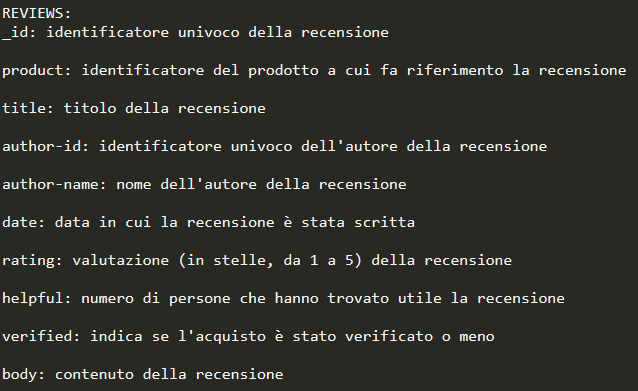
\includegraphics[width=0.9\linewidth]{img/reviewsAttributi.png}
\caption{\textit{reviews.json attributi}}
\end{figure}

\noindent Il dataset possiede gli attributi mostrati in tabella. Ogni record del dataset
è la rappresentazione di una singola recensione svolta da parte di un utente per
un certo prodotto nella data indicata.
Per l’identificazione dell’utente abbiamo a disposizione il campo author-name
e il campo author-id.
Per quanto riguarda i campi relativi alla recensione, abbiamo a disposizione body per il contenuto della recensione. La quasi totalità dell'elaborazione dei dati avverrà da questo campo.
Per identificare il prodotto abbiamo a disposizione solamente il campo asin, che
è un codice univoco.
Le recensioni sono classificate come verified se provengono da un acquisto su
Amazon tale che l'autore della recensione ha effettivamente acquistato il prodotto senza ricevere sconti particolari. Sono state selezionate solo quelle verified.

\begin{figure}[H]
	\centering
	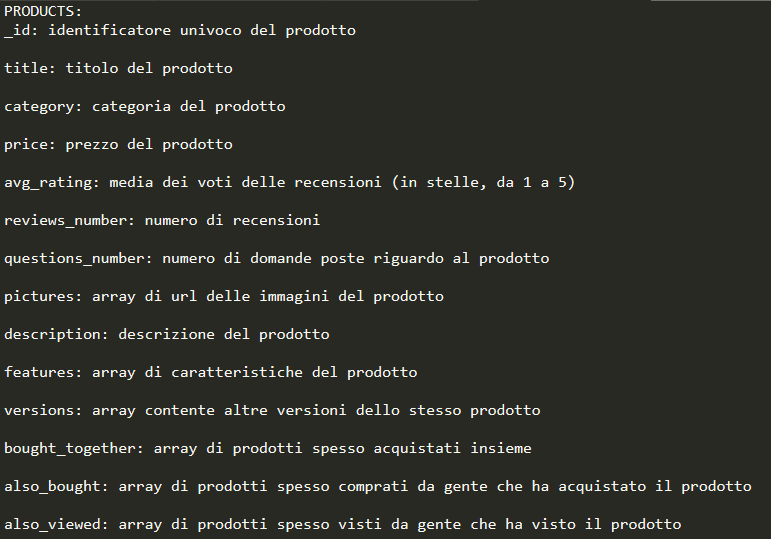
\includegraphics[width=0.9\linewidth]{img/productsAttributi.png}
	\caption{\textit{products.json attributi}}
\end{figure}

\noindent E' stato eseguito il left join delle tabelle linkando quindi i prodotti alle rispettive reviews attraverso gli indici "\_id" e "product".

\section{Sentiment analysis}
Il recupero di feedback dei clienti è un operazione estremamente importante per le aziende, soprattutto per le aziende leader che non badano a spese pagando miloni e milioni di euro per tale servizio. Per molto tempo si è fatto ciò manualmente (e tutt'ora per alcune aziende si procede in questo modo).

\noindent In questi anni però, vista l'ingente mole di informazioni, come ad esempio i feedback dei clienti, è fondamentale strutturare il raccoglimento dei dati e le loro analisi per il processo decisionale.

\noindent In particolare, per le opinioni su prodotti e servizi viene in aiuto la sentiment
analysis, una discplina che può fornire risposte riguardo le questioni più importanti dal punto di vista dei clienti. Il processo di sentiment analysis permette, attraverso l’elaborazione del linguaggio naturale, di estrarre e analizzare in modo automatizzato opinioni soggettive
espresse dall’utente, determinarne la polarità (positiva, neutrale, negativa) e,
successivamente, riassumerle in maniera da poter essere di valore per l’azienda.

\noindent In questo modo, le decisioni possono essere prese sulla base di una quantità di
dati significativa, piuttosto che da una semplice intuizione che non sempre si
rivela corretta.

\noindent La sentiment analysis è importante perché le aziende vogliono che il loro marchio sia recepito positivamente. A tal proposito, ci si può concentrare su commenti positivi o negativi oltre che sul feedback del cliente, per valutare sia i punti di forza che i punti su cui migliorare.

\newpage

\subsection{Preprocessing}
Prima di immergerci con l'aspect based sentiment analysis, è stato necessario
una fase di preprocessing.
Innanzitutto, si sono rimossi dal dataset i campi ritenuti superflui per l’analisi.

\noindent La manipolazione è avvenuta sequenzialmente e con step standard per analisi di questo tipo:
\begin{itemize}
	\item \textit{Divisione}: delle 10000 reviews si è andato a suddividere ciascuna in una lista di frasi attraverso la libreria di python NLTK;
	\item \textit{Tokenization}: per ogni frase si è andati a tokenizzarle per creare una lista di parole;
	\item \textit{Pulizia}: tutte le parole che fanno parte di punteggiatura, di simboli strani e di tutti quei elementi stopwords come articoli, congiunzioni che di fatto non aiutano a comprendere quello di cui si sta parlando;
	
	\noindent - Prima:\\
	\noindent ['Non', 'ho', 'mai', 'scritto', 'una', 'recensione', 'in', 'vita', 'mia', 'ma',
	'per', 'questo', 'gioco', 'sento', 'proprio', 'il', 'bisogno', 'di', 'scriverci'
	, 'qualcosa', '.'] \\
	
	\noindent - Dopo:\\
	\noindent ['mai', 'scritto', 'recensione', 'vita', 'gioco', 'sento', 'proprio', 'bisogno',
	'scriverci', 'qualcosa']
	
	\item \textit{Dizionario}: man mano che si scorrevano le parole si è costruito un dizionario necessario per poter eseguire ASUM;
	\item \textit{Indicizzazione}: per ogni parola delle frasi si è dovuto mappare la sua corrispettiva parola nel dizionario per generare BagOfSentences.txt, obbligatorio per ASUM come input. Di seguito un esempio di costruzione documento:
	\begin{figure}[H]
		\centering
		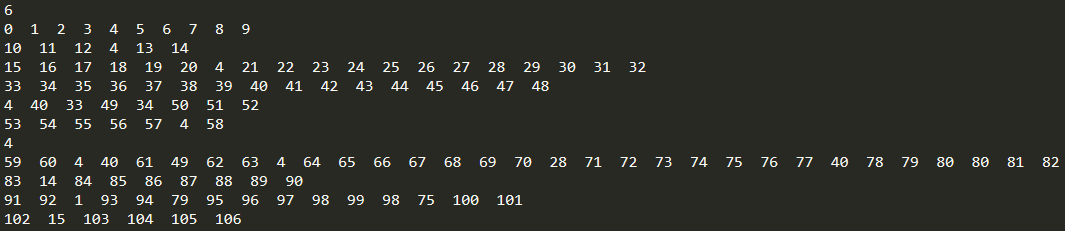
\includegraphics[width=0.9\linewidth]{img/inputBag.png}
		\caption{\textit{esempio input BagOfSentences.txt}}
	\end{figure}
	La prima riga indica il numero di frasi presenti nella review, di seguito infatti ci sono un numero di frasi in cui ogni indice si riferisce alla posizione della parola nella wordList;
	
	\item \textit{Output}: infine si è creato l'output WordList.txt e BagOfSentences.txt per mezzo della funzione to\_csv() della libreria Pandas.
\end{itemize}

\subsection{Creazione di Bag Of Sentencess}
Sono state rimosse dall’analisi le recensioni:
\begin{itemize}
	\item \textit{frasi lunghe}: con più di 300 parole;
	\item \textit{frasi corte}: con meno di 5 parole .
\end{itemize}

\newpage

\section{Analisi dei risultati}
L'output generato dal programma ASUM scritto in JAVA di Yohan Jo and Alice Oh restituisce diversi CSV, di cui a noi interessa quello relativo alle probabilità. Il nome dell'output dipende dalla stringa data in input. Infatti
STO2-T[t]-S[s]([d])-A[a]-B[b]-G[g]-I[i]-[variable].csv
dove:
\begin{itemize}
	\item \textit{t}: il numero di topics (aspetti);
	\item \textit{s}: numero di sentimenti;
	\item \textit{d}: numero di parole seed;
	\item \textit{a}: valore alpha simmetrico;
	\item \textit{b}: valore beta;
	\item \textit{g}: valore gamma;
	\item \textit{i}: numero di iterazioni di campionamento;
	\item \textit{variable}: variabile da inferire;
\end{itemize}

\begin{figure}[H]
	\centering
	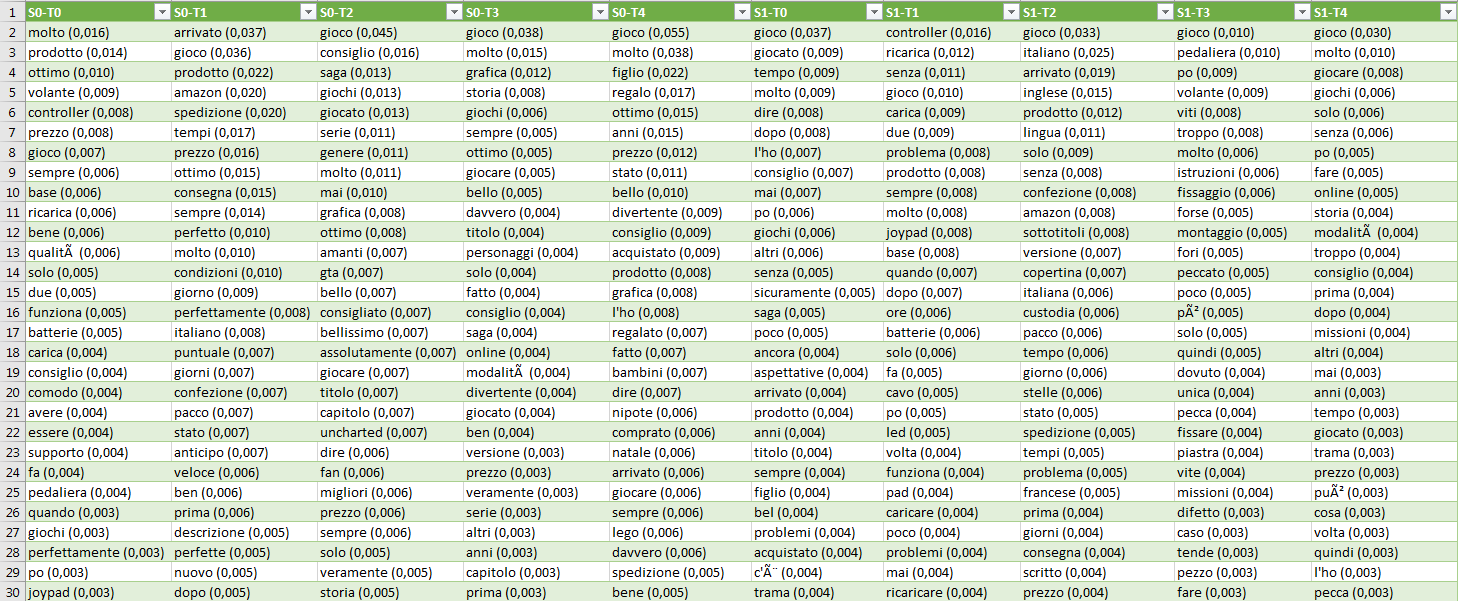
\includegraphics[width=0.9\linewidth]{img/outputASUM.png}
	\caption{\textit{output ASUM with -s 2 -t 5 -i 1000}}
\end{figure}

\noindent Di seguito vediamo l'output ottenuto con s = 2 e t = 5, cioè due sentimenti positivo e negativo e 5 aspetti di analisi. In ogni colonna visualizziamo le parole con una probabilità decrescente andando dall'alto verso il basso.

\begin{figure}[H]
	\centering
	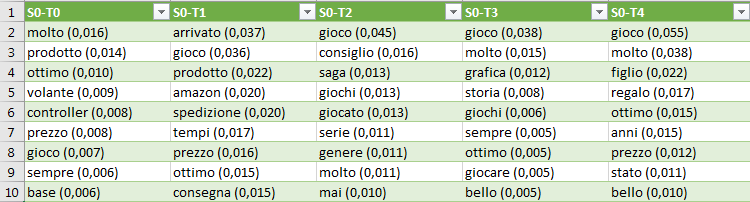
\includegraphics[width=0.9\linewidth]{img/outputASUM0.png}
	\caption{\textit{output ASUM s 0}}
\end{figure}

\noindent Focalizzandoci nell'area in cui abbiamo i valori positivi possiamo notare che compaiono parole che infatti hanno un valore positivo. Notiamo che dal momento che trattiamo dei videogiochi compare per 3 topic su 5 come prima parola "gioco" con una probabilità maggiore di 0.037. 

\begin{figure}[H]
	\centering
	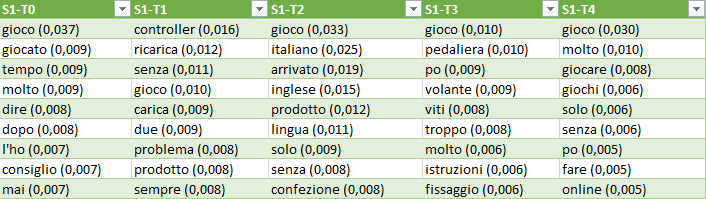
\includegraphics[width=0.9\linewidth]{img/outputASUM1.png}
	\caption{\textit{output ASUM s 1}}
\end{figure}

\noindent Focalizzandoci nell'area in cui abbiamo i valori negativi possiamo notare che compaiono parole che oscillano tra un valore positivo e valore negativo. Il problema principale deriva dalla lingua utilizzata. Notiamo che la parola gioco è predominante ancora con una percentuale mediamente più bassa. Notiamo che nonostante sia stato fatto con regex l'eliminazione di parole con l'apostrofo una è riuscita a passare lo stesso "l'ho", probabilmente un apostrofo con una formattazione diversa

\section{Conclusioni}
L’esplorazione delle recensioni di prodotti Amazon ha permesso di visualizzare un buon numero di informazioni che possono essere estratte da opinioni degli acquirenti con lo scopo di stilare statistiche e valutazioni e poter quindi prendere decisioni in ambito aziendale per migliorare i servizi offerti o centrare meglio la
propria clientela. Tali tecniche sono più affinate per il linguaggio inglese, pertanto bisogna intervenire con un miglior preprocessing e con un numero di SentiWords più idoneo e di qualità.


\end{document}